\documentclass[preview,convert={convertexe={magick},outext=.ps}]{standalone}
\usepackage[dvipdfm]{geometry}

%graphics
\usepackage{xcolor}
\usepackage{tikz}
\usetikzlibrary{shapes.geometric, shapes.multipart, arrows, calc, through,intersections}
\usepackage[caption=false,font=footnotesize]{subfig}

\begin{document}
    

\begin{figure}[!t]
\centering
\subfloat[2DD]{
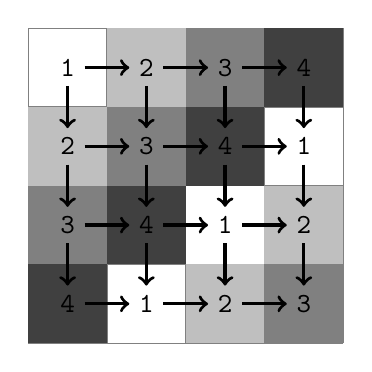
\begin{tikzpicture}[
cell label/.style = {text centered}
]

\draw[step=1cm,gray,thin] (0,0) grid (4,4);

\fill[lightgray] (0,2) rectangle (1,3);
\fill[lightgray] (1,3) rectangle (2,4);

\fill[gray] (0,1) rectangle (1,2);
\fill[gray] (1,2) rectangle (2,3);
\fill[gray] (2,3) rectangle (3,4);

\fill[darkgray] (0,0) rectangle (1,1);
\fill[darkgray] (1,1) rectangle (2,2);
\fill[darkgray] (2,2) rectangle (3,3);
\fill[darkgray] (3,3) rectangle (4,4);

\fill[lightgray]   (2,0) rectangle (3,1);
\fill[lightgray]   (3,1) rectangle (4,2);

\fill[gray] (3,0) rectangle (4,1);

\node (03) at (0.5, 3.5) [cell label] {$\mathtt1$};

\node (02) at (0.5, 2.5) [cell label] {$\mathtt2$};
\node (13) at (1.5, 3.5) [cell label] {$\mathtt2$};

\node (01) at (0.5, 1.5) [cell label] {$\mathtt3$};
\node (12) at (1.5, 2.5) [cell label] {$\mathtt3$};
\node (23) at (2.5, 3.5) [cell label] {$\mathtt3$};

\node (00) at (0.5, 0.5) [cell label] {$\mathtt4$};
\node (11) at (1.5, 1.5) [cell label] {$\mathtt4$};
\node (22) at (2.5, 2.5) [cell label] {$\mathtt4$};
\node (33) at (3.5, 3.5) [cell label] {$\mathtt4$};

\node (10) at (1.5, 0.5) [cell label] {$\mathtt1$};
\node (21) at (2.5, 1.5) [cell label] {$\mathtt1$};
\node (32) at (3.5, 2.5) [cell label] {$\mathtt1$};

\node (20) at (2.5, 0.5) [cell label] {$\mathtt2$};
\node (31) at (3.5, 1.5) [cell label] {$\mathtt2$};

\node (30) at (3.5, 0.5) [cell label] {$\mathtt3$};

\draw[->, very thick] (03.east) -- (13.west);
\draw[->, very thick] (13.east) -- (23.west);
\draw[->, very thick] (23.east) -- (33.west);

\draw[->, very thick] (02.east) -- (12.west);
\draw[->, very thick] (12.east) -- (22.west);
\draw[->, very thick] (22.east) -- (32.west);

\draw[->, very thick] (01.east) -- (11.west);
\draw[->, very thick] (11.east) -- (21.west);
\draw[->, very thick] (21.east) -- (31.west);

\draw[->, very thick] (00.east) -- (10.west);
\draw[->, very thick] (10.east) -- (20.west);
\draw[->, very thick] (20.east) -- (30.west);

\draw[->, very thick] (03.south) -- (02.north);
\draw[->, very thick] (02.south) -- (01.north);
\draw[->, very thick] (01.south) -- (00.north);

\draw[->, very thick] (13.south) -- (12.north);
\draw[->, very thick] (12.south) -- (11.north);
\draw[->, very thick] (11.south) -- (10.north);

\draw[->, very thick] (23.south) -- (22.north);
\draw[->, very thick] (22.south) -- (21.north);
\draw[->, very thick] (21.south) -- (20.north);

\draw[->, very thick] (33.south) -- (32.north);
\draw[->, very thick] (32.south) -- (31.north);
\draw[->, very thick] (31.south) -- (30.north);
\end{tikzpicture}
}
\subfloat[USE]{
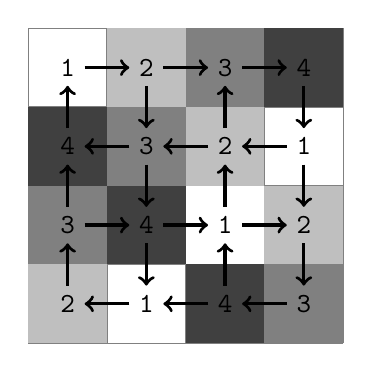
\begin{tikzpicture}[
cell label/.style = {text centered}
]

\draw[step=1cm,gray,thin] (0,0) grid (4,4);

\fill[lightgray] (0,0) rectangle (1,1);
\fill[darkgray] (2,0) rectangle (3,1);
\fill[gray]   (3,0) rectangle (4,1);

\fill[lightgray] (3,1) rectangle (4,2);
\fill[darkgray] (1,1) rectangle (2,2);
\fill[gray]   (0,1) rectangle (1,2);

\fill[lightgray] (2,2) rectangle (3,3);
\fill[darkgray] (0,2) rectangle (1,3);
\fill[gray]   (1,2) rectangle (2,3);

\fill[lightgray] (1,3) rectangle (2,4);
\fill[darkgray] (3,3) rectangle (4,4);
\fill[gray]   (2,3) rectangle (3,4);

\node (00) at (0.5, 0.5) [cell label] {$\mathtt2$};
\node (10) at (1.5, 0.5) [cell label] {$\mathtt1$};
\node (20) at (2.5, 0.5) [cell label] {$\mathtt4$};
\node (30) at (3.5, 0.5) [cell label] {$\mathtt3$};

\node (01) at (0.5, 1.5) [cell label] {$\mathtt3$};
\node (11) at (1.5, 1.5) [cell label] {$\mathtt4$};
\node (21) at (2.5, 1.5) [cell label] {$\mathtt1$};
\node (31) at (3.5, 1.5) [cell label] {$\mathtt2$};

\node (02) at (0.5, 2.5) [cell label] {$\mathtt4$};
\node (12) at (1.5, 2.5) [cell label] {$\mathtt3$};
\node (22) at (2.5, 2.5) [cell label] {$\mathtt2$};
\node (32) at (3.5, 2.5) [cell label] {$\mathtt1$};

\node (03) at (0.5, 3.5) [cell label] {$\mathtt1$};
\node (13) at (1.5, 3.5) [cell label] {$\mathtt2$};
\node (23) at (2.5, 3.5) [cell label] {$\mathtt3$};
\node (33) at (3.5, 3.5) [cell label] {$\mathtt4$};

\draw[->, very thick] (03.east) -- (13.west);
\draw[->, very thick] (13.east) -- (23.west);
\draw[->, very thick] (23.east) -- (33.west);

\draw[->, very thick] (01.east) -- (11.west);
\draw[->, very thick] (11.east) -- (21.west);
\draw[->, very thick] (21.east) -- (31.west);

\draw[->, very thick] (32.west) -- (22.east);
\draw[->, very thick] (22.west) -- (12.east);
\draw[->, very thick] (12.west) -- (02.east);

\draw[->, very thick] (30.west) -- (20.east);
\draw[->, very thick] (20.west) -- (10.east);
\draw[->, very thick] (10.west) -- (00.east);

\draw[->, very thick] (00.north) -- (01.south);
\draw[->, very thick] (01.north) -- (02.south);
\draw[->, very thick] (02.north) -- (03.south);

\draw[->, very thick] (20.north) -- (21.south);
\draw[->, very thick] (21.north) -- (22.south);
\draw[->, very thick] (22.north) -- (23.south);

\draw[->, very thick] (13.south) -- (12.north);
\draw[->, very thick] (12.south) -- (11.north);
\draw[->, very thick] (11.south) -- (10.north);

\draw[->, very thick] (33.south) -- (32.north);
\draw[->, very thick] (32.south) -- (31.north);
\draw[->, very thick] (31.south) -- (30.north);
\end{tikzpicture}
\label{fig:use}
}
\end{figure}
\end{document}
